% !TEX root = Skin_Lesion_Classification_Using_Machine_Learning.tex

\section{Handling of Unknown Data [SE]}\label{sec:unknown_data}

As mentioned in section \ref{sec:introduction}, the test dataset contains images that don't belong to any of the categories of the training dataset. There is no information about the number of unknown images, the only given information is, that these images still show human skin and skin lesions. The performance of our models on the test dataset was not revealed before the submission deadline. That conditions made it hard to tune the testset classification accuracy. 

The automated evaluation system for this challenge required for each image a vector where each element is equal to the estimated probability for the respective class. In contrast to the real ISIC 2019 challenge, this vector is supposed to sum up to $1$. For that reason it was obvious to use a softmax activation function for the neural network approach. We assumed that the maximum value of the predicted class probabilities (referred to as confidence in the following) will be low for images of the unknown category. Literature sows that this assumption is not necessary true \cite{softmax_conf}. To test if this approach is still usable in this situation, we set all images showing basal cell carcinoma (class $2$) to unknown and trained the model on the remaining seven categories. 

\begin{figure}[h]
    \centering
    % include first image
    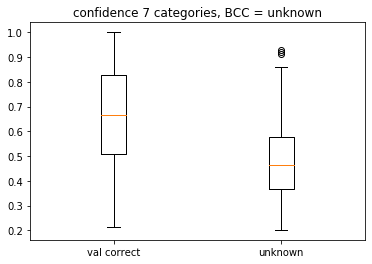
\includegraphics[width=.75\linewidth]{pictures/box_unknown.png}  
    \caption{comparison of distribution of confidence for known and unknown images}
    \label{fig:box_unknown}
\end{figure}
% #TODO maybe use hist or create better plot
Figure \ref{fig:box_unknown} shows the result of this test. The bar for "val correct" referrers to the confidence values for the correctly classified images in the validation dataset, "unknown" to the confidence for the images of the class that was set to unknown. It can be seen, that our assumption holds for this test. The confidence for unknown images is in average significantly lower. Both classes are however not perfectly separated. With no additional information it is not easy to assign a threshold for the confidence under which the lesion is assumed to be unknown. With no feedback for the performance on the test dataset we didn't see any evaluation method that would allow us to optimize this hyperparameter. 
Given the time constraints however, we decided that this approach is the best method available for us to handle the unknown class. 

We wanted to use this approach also in phase one using a SVM but the SVC class in sklearn does only predict classes and does not output probabilities for them. The \verb|predict_proba| method wich can for other classifiers output probability estimates was not applicable for SVMs. It uses Platt scaling and internal cross validation to create probabilities \cite{scikit-learn}. However they are not consistent with the normal class estimations and produced much worse results. For that reason we followed the advice in the documentation and used the values of the decision function for our confidence threshold. 
